% Aalto Master's Thesis template
% Compatible with: UTF-8, pdflatex, biblatex, biber
%
% Compile using the following commands:
% $ pdflatex thesis.tex
% $ biber thesis
% $ pdflatex thesis.tex
% $ pdflatex thesis.tex
% $ pdflatex thesis.tex
%

\documentclass[12pt,a4paper,oneside,pdftex]{report}

\usepackage[utf8]{inputenc}
\usepackage[T1]{fontenc}
\usepackage[finnish,swedish,english]{babel}

% Font selection
%\usepackage{palatino}
%\usepackage[sc]{mathpazo}
\usepackage{kpfonts}
%\usepackage{tgpagella}
%\usepackage{garamond}
%\usepackage{lmodern}


% Verbatim provides a standard teletype environment that renderes
% the text exactly as written in the tex file. Useful for code
% snippets (although you can also use the listings package to get
% automatic code formatting).
\usepackage{verbatim}

% Longtable provides a tabular environment that can span multiple
% pages. This is used in the example abbreviations file.
\usepackage{longtable}

% The titlesec package can be used to alter the look of the titles
% of sections, chapters, and so on. This example uses the ``medium''
% package option which sets the titles to a medium size, making them
% a bit smaller than what is the default. You can fine-tune the
% title fonts and sizes by using the package options. See the package
% documentation.
\usepackage[medium]{titlesec}

% The TikZ package allows you to create professional technical figures.
% The learning curve is quite steep, but it is definitely worth it if
% you wish to have really good-looking technical figures.
\usepackage{tikz}
% You also need to specify which TikZ libraries you use
\usetikzlibrary{positioning}
\usetikzlibrary{calc}
\usetikzlibrary{arrows}
\usetikzlibrary{decorations.pathmorphing,decorations.markings}
\usetikzlibrary{shapes}
\usetikzlibrary{patterns}

% Microtype for better typography
\usepackage[stretch=30,protrusion=true,final,expansion,tracking=true,kerning,spacing]{microtype}

% SI units. See table in 2lorem.tex for example
\usepackage{siunitx}
\sisetup{
    alsoload=binary
}

% Publication quality tables. See table in 2lorem.tex for example
\usepackage{booktabs}

% Use biber instead of bibtex as it supports UTF-8 among other things
\usepackage[backend=biber,style=numeric-verb,sortcites=true,sorting=none]{biblatex}

% Nicer looking caption for figures, tables, etc.
\usepackage[labelfont={bf},textfont={it}]{caption}

% Multiple figures inside one figure. See figure in 1lipsum.tex for example
\usepackage{subfig}

% Inconsolata monospace font for verbatim environment
\usepackage{inconsolata}

% For rotating figures
\usepackage{rotating}

% Separate multiple citations with space instead of comma
% E.g. "[1] [2] [3]" instead of "[1], [2], [3]"
\renewcommand\multicitedelim{\space}

% Prevent orphan and widow rows
\widowpenalty=10000
\clubpenalty=10000

% Bibliography
\addbibresource{sources.bib}

% The aalto-thesis package provides typesetting instructions for the
% standard master's thesis parts (abstracts, front page, and so on)
% Load this package second-to-last, just before the hyperref package.
% Options that you can use:
%   mydraft - renders the thesis in draft mode.
%             Do not use for the final version.
%   doublenumbering - [optional] number the first pages of the thesis
%                     with roman numerals (i, ii, iii, ...); and start
%                     arabic numbering (1, 2, 3, ...) only on the
%                     first page of the first chapter
%   twoinstructors  - changes the title of instructors to plural form
%   twosupervisors  - changes the title of supervisors to plural form
%\usepackage[mydraft,doublenumbering]{aalto-thesis}
\usepackage[doublenumbering]{aalto-thesis}


% Hyperref
% ------------------------------------------------------------------
% Hyperref creates links from URLs, for references, and creates a
% TOC in the PDF file.
% This package must be the last one you include, because it has
% compatibility issues with many other packages and it fixes
% those issues when it is loaded.
\RequirePackage[pdftex]{hyperref}
% Setup hyperref so that links are clickable but do not look
% different
\hypersetup{colorlinks=false,raiselinks=false,breaklinks=true}
\hypersetup{pdfborder={0 0 0}}
\hypersetup{bookmarksnumbered=true}
% The following line suggests the PDF reader that it should show the
% first level of bookmarks opened in the hierarchical bookmark view.
\hypersetup{bookmarksopen=true,bookmarksopenlevel=1}
% Hyperref can also set up the PDF metadata fields. These are
% set a bit later on, after the thesis setup.


% Thesis setup
% ==================================================================
% Change these to fit your own thesis.
% \COMMAND always refers to the English version;
% \FCOMMAND refers to the Finnish version; and
% \SCOMMAND refers to the Swedish version.
% You may comment/remove those language variants that you do not use
% (but then you must not include the abstracts for that language)
% ------------------------------------------------------------------
% If you do not find the command for a text that is shown in the cover page or
% in the abstract texts, check the aalto-thesis.sty file and locate the text
% from there.
% All the texts are configured in language-specific blocks (lots of commands
% that look like this: \renewcommand{\ATCITY}{Espoo}.
% You can just fix the texts there. Just remember to check all the language
% variants you use (they are all there in the same place).
% ------------------------------------------------------------------
\newcommand{\TITLE}{Lorem Ipsum} % TODO
\newcommand{\FTITLE}{Lorem Ipsum} % TODO
\newcommand{\SUBTITLE}{}
\newcommand{\FSUBTITLE}{}
\newcommand{\DATE}{1.1.2012} % TODO
\newcommand{\FDATE}{1.1.2012} % TODO

% Supervisors and instructors
% ------------------------------------------------------------------
% If you have two supervisors, write both names here, separate them with a
% double-backslash (see below for an example)
% Also remember to add the package option ``twosupervisors'' or
% ``twoinstructors'' to the aalto-thesis package so that the titles are in
% plural.
% Example of one supervisor:
%\newcommand{\SUPERVISOR}{Professor Antti Ylä-Jääski}
%\newcommand{\FSUPERVISOR}{Professori Antti Ylä-Jääski}
%\newcommand{\SSUPERVISOR}{Professor Antti Ylä-Jääski}
\newcommand{\SUPERVISOR}{Prof. John Doe} % TODO
\newcommand{\FSUPERVISOR}{Prof. John Doe} % TODO
\newcommand{\SSUPERVISOR}{Prof. John Doe} % TODO

% If you have only one instructor, just write one name here
\newcommand{\INSTRUCTOR}{Jane Doe M.Sc. (Tech.)} % TODO
\newcommand{\FINSTRUCTOR}{DI Jane Doe} % TODO
\newcommand{\SINSTRUCTOR}{DI Jane Doe} % TODO
% If you have two instructors, separate them with \\ to create linefeeds
% \newcommand{\INSTRUCTOR}{Olli Ohjaaja M.Sc. (Tech.)\\
%  Elli Opas M.Sc. (Tech)}
%\newcommand{\FINSTRUCTOR}{Diplomi-insinööri Olli Ohjaaja\\
%  Diplomi-insinööri Elli Opas}
%\newcommand{\SINSTRUCTOR}{Diplomingenjör Olli Ohjaaja\\
%  Diplomingenjör Elli Opas}

% If you have two supervisors, it is common to write the schools
% of the supervisors in the cover page. If the following command is defined,
% then the supervisor names shown here are printed in the cover page. Otherwise,
% the supervisor names defined above are used.
%\newcommand{\COVERSUPERVISOR}{Professor Antti Ylä-Jääski, Aalto University\\
%  Professor Pekka Perustieteilijä, University of Helsinki}

% The same option is for the instructors, if you have multiple instructors.
% \newcommand{\COVERINSTRUCTOR}{Olli Ohjaaja M.Sc. (Tech.), Aalto University\\
%  Elli Opas M.Sc. (Tech), Aalto SCI}


% Other stuff
% ------------------------------------------------------------------
\newcommand{\PROFESSORSHIP}{Information and Computer Systems in Automation} % TODO
\newcommand{\FPROFESSORSHIP}{Automaation tietotekniikka} % TODO check
% Professorship code is the same in all languages
\newcommand{\PROFCODE}{AS-116} % TODO check
\newcommand{\KEYWORDS}{Thesis template, master's thesis} % TODO
\newcommand{\FKEYWORDS}{Diplomityöpohja} % TODO
\newcommand{\LANGUAGE}{English} % TODO
\newcommand{\FLANGUAGE}{Englanti} % TODO

% Author is the same for all languages
\newcommand{\AUTHOR}{Jane Roe}

% Currently the English versions are used for the PDF file metadata
% Set the PDF title
\hypersetup{pdftitle={\TITLE\ \SUBTITLE}}
% Set the PDF author
\hypersetup{pdfauthor={\AUTHOR}}
% Set the PDF keywords
\hypersetup{pdfkeywords={\KEYWORDS}}
% Set the PDF subject
\hypersetup{pdfsubject={Master's Thesis}}


% Layout settings
% ------------------------------------------------------------------

% When you write in English, you should use the standard LaTeX
% paragraph formatting: paragraphs are indented, and there is no
% space between paragraphs.
% When writing in Finnish, we often use no indentation in the
% beginning of the paragraph, and there is some space between the
% paragraphs.

% If you write your thesis Finnish, uncomment these lines; if
% you write in English, leave these lines commented!
%\setlength{\parindent}{0pt}
%\setlength{\parskip}{1ex}

% Use this to control how much space there is between each line of text.
% 1 is normal (no extra space), 1.3 is about one-half more space, and
% 1.6 is about double line spacing.
\linespread{1.05}
% \linespread{1.3}

% Extra hyphenation settings
% ------------------------------------------------------------------
% You can list here all the files that are not hyphenated correctly.
% You can provide many \hyphenation commands and/or separate each word
% with a space inside a single command. Put hyphens in the places where
% a word can be hyphenated.
% Note that (by default) LaTeX will not hyphenate words that already
% have a hyphen in them (for example, if you write ``structure-modification
% operation'', the word structure-modification will never be hyphenated).
% You need a special package to hyphenate those words.
%\hyphenation{di-gi-taa-li-sta}


% Proper style for book binding, left margin bigger than right margin
% Uncomment to take into use
%\setlength{\parindent}{0pt}
%\setlength{\parskip}{2ex}
%\setlength{\textwidth}{140mm}
%\setlength{\oddsidemargin}{20mm}
%\setlength{\evensidemargin}{20mm}
%\setlength{\textheight}{240mm}
%\setlength{\voffset}{3mm}
%\setlength{\topmargin}{-11mm}


% The preamble ends here, and the document begins.
% Place all formatting commands and such before this line.
% ------------------------------------------------------------------
\begin{document}
% This command adds a PDF bookmark to the cover page. You may leave
% it out if you don't like it...
\pdfbookmark[0]{Cover}{bookmark.0.cover}
% This command is defined in aalto-thesis.sty. It controls the page
% numbering based on whether the doublenumbering option is specified
\startcoverpage

% Cover page
% ------------------------------------------------------------------
% Options: finnish, english, and swedish
% These control in which language the cover-page information is shown
\coverpage{english} % TODO


% Abstracts
% ------------------------------------------------------------------
% Include an abstract in the language that the thesis is written in,
% and if your native language is Finnish or Swedish, one in that language.

% Abstract in English
% ------------------------------------------------------------------
\thesisabstract{english}{
In id fringilla velit. Maecenas sed ante sit amet nisi iaculis bibendum sed vel
elit. Quisque eleifend lacus nec ipsum lobortis ornare. Nam lectus diam,
facilisis eget porttitor ac, fringilla quis massa. Phasellus ac dolor sem, eget
varius lacus. Sed sit amet ipsum eget arcu tristique aliquam. Integer aliquam
velit sit amet odio tempus commodo. Quisque commodo lacus in leo sagittis vel
dignissim quam vestibulum. Cras fringilla velit et diam dictum faucibus.
Pellentesque at eros non mauris auctor euismod. Nullam convallis arcu vel lectus
sollicitudin rutrum. Praesent consequat, nisl at pretium posuere, neque arcu
dapibus lacus, ut sollicitudin elit velit ultricies libero. Vestibulum ante
ipsum primis in faucibus orci luctus et ultrices posuere cubilia Curae;

Nulla semper hendrerit molestie. Pellentesque blandit velit sit amet est
vestibulum faucibus. Nullam massa turpis, venenatis non mollis fringilla, mattis
et diam. Fusce molestie convallis elementum. Morbi nec lacus dapibus arcu mollis
gravida. Aliquam erat volutpat. Nam vitae magna nunc. Nunc ut ipsum at massa
porttitor vestibulum. Praesent diam lorem, ultrices nec vestibulum id, volutpat
nec lacus.
}

% Abstract in Finnish
% ------------------------------------------------------------------
\thesisabstract{finnish}{
Cras tincidunt bibendum erat, vel tincidunt diam porttitor aliquam. Donec sit
amet urna non felis placerat pharetra. Aenean ultrices facilisis nulla vitae
semper. Nullam non libero quis dui fermentum aliquam id vel eros. Praesent
elementum tortor quis sem congue iaculis sit amet eget nisl. Quisque erat
tortor, condimentum eu volutpat et, blandit et augue. Phasellus erat turpis,
pretium non feugiat id, posuere id velit. Vestibulum ut sapien felis, quis
convallis dui.

In elementum est eu nulla hendrerit feugiat. In sodales diam vel lacus cursus
tincidunt. Morbi nibh dui, imperdiet non vestibulum non, dignissim id risus. Sed
sollicitudin neque lectus, porttitor sollicitudin elit. Nulla facilisi. Nullam
in ante eu mi suscipit sollicitudin. Sed est velit, gravida facilisis varius
eget, tempus sed urna. Aliquam erat volutpat. Nam semper condimentum nisi.
Nullam scelerisque, metus nec sodales vulputate, purus augue venenatis urna, sit
amet mattis turpis nisl ac metus. Mauris nec odio ut neque condimentum vulputate
vel in turpis. Nulla facilisi. Nulla id tellus sapien, vitae blandit lorem.
}

% Acknowledgements
% ------------------------------------------------------------------
% Select the language you use in your acknowledgements
\selectlanguage{english}

% Uncomment this line if you wish acknoledgements to appear in the
% table of contents
%\addcontentsline{toc}{chapter}{Acknowledgements}

% The star means that the chapter isn't numbered and does not
% show up in the TOC
\chapter*{Acknowledgements} % TODO
In id fringilla velit. Maecenas sed ante sit amet nisi iaculis bibendum sed vel
elit. Quisque eleifend lacus nec ipsum lobortis ornare. Nam lectus diam,
facilisis eget porttitor ac, fringilla quis massa. Phasellus ac dolor sem, eget
varius lacus. Sed sit amet ipsum eget arcu tristique aliquam. Integer aliquam
velit sit amet odio tempus commodo. Quisque commodo lacus in leo sagittis vel
dignissim quam vestibulum. Cras fringilla velit et diam dictum faucibus.
Pellentesque at eros non mauris auctor euismod. Nullam convallis arcu vel lectus
sollicitudin rutrum. Praesent consequat, nisl at pretium posuere, neque arcu
dapibus lacus, ut sollicitudin elit velit ultricies libero. Vestibulum ante
ipsum primis in faucibus orci luctus et ultrices posuere cubilia Curae;

\vskip 10mm

\noindent Espoo, \DATE
\vskip 5mm
\noindent\AUTHOR

% Acronyms
% ------------------------------------------------------------------
% Use \cleardoublepage so that IF two-sided printing is used
% (which is not often for masters theses), then the pages will still
% start correctly on the right-hand side.
\cleardoublepage
% Example acronyms are placed in a separate file, abbreviations.tex
\addcontentsline{toc}{chapter}{Abbreviations}
\chapter*{Abbreviations}

% The longtable environment should break the table properly to multiple pages,
% if needed

\noindent
\begin{longtable}{@{}p{0.25\textwidth}p{0.7\textwidth}@{}}
LI & Lorem Ipsum \\
ABC & Quisque et mi lacus, nec porta ante. \\
DEF & Proin pellentesque accumsan laoreet \\
\end{longtable}



% Table of contents
% ------------------------------------------------------------------
\cleardoublepage
% This command adds a PDF bookmark that links to the contents.
% You can use \addcontentsline{} as well, but that also adds contents
% entry to the table of contents, which is kind of redundant.
% The text ``Contents'' is shown in the PDF bookmark.
\pdfbookmark[0]{Table of contents}{bookmark.0.contents}
\tableofcontents

% List of tables
% ------------------------------------------------------------------
% You only need a list of tables for your thesis if you have very
% many tables. If you do, uncomment the following two lines.
% \cleardoublepage
% \listoftables

% Table of figures
% ------------------------------------------------------------------
% You only need a list of figures for your thesis if you have very
% many figures. If you do, uncomment the following two lines.
% \cleardoublepage
% \listoffigures

% The following label is used for counting the prelude pages
\label{pages-prelude}
\cleardoublepage

%%%%%%%%%%%%%%%%% The main content starts here %%%%%%%%%%%%%%%%%%%%%
% ------------------------------------------------------------------
% This command is defined in aalto-thesis.sty. It controls the page
% numbering based on whether the doublenumbering option is specified
\startfirstchapter

% Add headings to pages (the chapter title is shown)
\pagestyle{headings}

% The contents of the thesis are separated to their own files.
% Edit the content in these files, rename them as necessary.
% ------------------------------------------------------------------
\chapter{Introduction}
\label{section:introduction}

Lorem ipsum dolor sit amet, consectetur adipiscing elit. Phasellus justo eros,
rutrum sed pretium nec, venenatis id arcu. Nunc aliquam sollicitudin massa nec
aliquet. Cras felis lorem, viverra et consequat a, posuere rhoncus odio. Duis
commodo tincidunt metus vitae luctus. Phasellus in odio a velit aliquet
elementum sit amet convallis purus. Nulla at nulla justo. Proin eros turpis,
rutrum eget semper nec, pharetra ut sem. Ut rhoncus purus sed orci porttitor at
auctor turpis ornare. Donec felis elit, mollis vulputate tempus a, rutrum et
justo. Morbi convallis lacus egestas nulla auctor mollis. Fusce erat mauris,
consectetur ac lacinia quis, fringilla non nunc.

Aliquam et metus sed odio bibendum venenatis. Integer ut volutpat magna.
Phasellus eleifend eleifend nunc vel tempor. Nam imperdiet nibh quis magna
congue sit amet eleifend nunc rutrum. In hac habitasse platea dictumst. Etiam
pretium, enim non accumsan vulputate, ante tortor sollicitudin lorem, non
consequat erat odio commodo massa~\ref{section:introduction:structure}.
Phasellus cursus enim quis risus varius in tempor justo lacinia. Integer
consectetur ultricies neque ac vehicula. Sed blandit, metus id tincidunt
volutpat, turpis dolor hendrerit augue, in congue augue risus sit amet libero.
Suspendisse varius rhoncus dolor, a ornare nisl dignissim eget.

\section{Thesis structure}
\label{section:introduction:structure}

Nullam nec eleifend turpis. Donec a libero non ante imperdiet convallis quis et
mi. Nam eu massa quis arcu tempor pulvinar. Maecenas sed mauris purus. Integer a
justo sit amet felis dapibus rhoncus. Maecenas vulputate lacinia neque, vel
eleifend eros lacinia quis. Aliquam nec felis erat. Morbi eget dictum nulla.
Nulla sapien lorem, rutrum eget tempor vel, euismod a urna. Quisque porttitor,
libero quis sollicitudin sollicitudin, neque felis auctor arcu, vel varius
libero ligula at urna. Donec lectus nisi, convallis sit amet cursus eu, tempus
eu arcu. Vestibulum quis urna risus, vitae faucibus eros. Sed cursus interdum
eros ut convallis. Donec in purus id ligula dignissim dictum. Morbi ipsum
libero, gravida id vestibulum vehicula, eleifend dapibus arcu. Proin eget nunc
et velit pellentesque vulputate.

Vivamus vestibulum semper euismod. Praesent vulputate libero in dui fringilla at
tempor lorem vestibulum. Etiam tincidunt nibh nec magna dapibus et pretium justo
scelerisque. Donec id felis augue. In ut risus dolor, sit amet lobortis magna.
Pellentesque ac odio et mi aliquet consequat vel non nibh. Vivamus interdum
lacinia interdum. Fusce ut elit urna. Morbi quis scelerisque mauris. Donec
semper purus erat. Phasellus id metus neque. Donec eu pellentesque risus.

Sed tempor tortor sed sem consequat blandit. Aliquam erat volutpat. Pellentesque
porttitor velit in nisi posuere ac adipiscing justo rutrum. Aliquam aliquet elit
in mauris laoreet dignissim. Duis lacus purus, blandit sit amet placerat at,
pulvinar eu ipsum. Aenean eu enim non justo accumsan aliquet eget nec dolor.
Nullam vitae dui et urna fermentum adipiscing. Integer a mi est. Nam non eros
quis felis condimentum vestibulum. Pellentesque habitant morbi tristique
senectus et netus et malesuada fames ac turpis egestas.



\chapter{Lipsum}
\label{section:lipsum}

Cras pharetra bibendum felis nec fringilla. Curabitur accumsan iaculis justo, eget imperdiet erat malesuada sed. Quisque lorem eros, feugiat sollicitudin adipiscing at, rutrum quis elit. Nulla non nisl nunc. Fusce vitae tortor non enim vestibulum suscipit in imperdiet elit. Curabitur sit amet leo purus, quis ornare dui. Suspendisse vel arcu vel diam iaculis adipiscing a sit amet mauris. Vestibulum augue magna, placerat vitae sagittis in, iaculis quis sem. Proin ut arcu pulvinar orci blandit iaculis. Etiam mauris lacus, luctus a dictum vel, rhoncus non dui. Mauris est urna, varius eget egestas a, adipiscing nec odio. Aenean iaculis nisi sed quam pretium aliquet. Quisque et mi lacus, nec porta ante. Nunc sed ante id diam hendrerit interdum in vitae eros. Ut odio ligula, commodo id volutpat non, tristique at odio.

\section{Cras pharetra bibendum}
\label{section:lipsum:cras}

Ut vitae nulla vel purus egestas tincidunt sit amet at tellus. Lorem ipsum dolor sit amet, consectetur adipiscing elit. Praesent et libero elit. Curabitur vel nulla odio, a eleifend arcu. Mauris dolor velit, aliquam ac mattis eu, cursus vitae mauris. Vestibulum at eleifend purus. Phasellus fringilla nulla a augue sollicitudin dignissim. Pellentesque et ligula vel nulla condimentum semper. Aliquam imperdiet dapibus fermentum. Nam ut diam dui. Sed malesuada auctor erat in viverra. Integer nisl augue, imperdiet non pellentesque ac, vehicula quis elit. Suspendisse varius tellus non nibh ornare ac consequat sapien adipiscing. Vivamus in tempus tellus. Aliquam erat volutpat. Morbi orci felis, venenatis tempus sodales ut, aliquam viverra justo.~\cite{conference:06,Doe:2010}

\begin{figure}[ht]
	\centering
	\subfloat[Something]{
		\resizebox{0.45\linewidth}{!}{
			\label{figure:some1}
			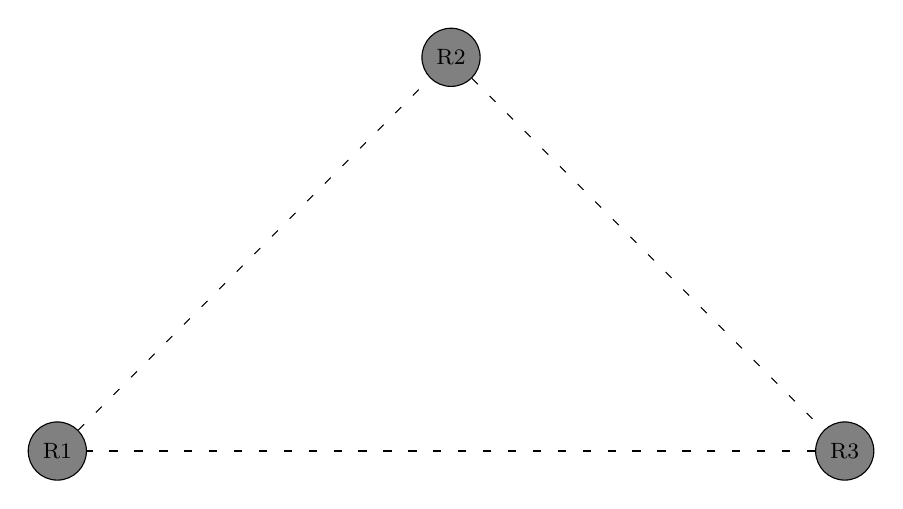
\begin{tikzpicture}[auto,node distance=3cm,on grid]
	\tikzstyle{round} = [draw,circle,minimum size=20pt,font=\footnotesize,fill=gray]
	\tikzstyle{link} = [loosely dashed]

	\node[round] at (0,0) (r1) {R1};
	\node[round] at (5,5) (r2) {R2};
	\node[round] at (10,0) (r3) {R3};

	\begin{scope}[link]
		\draw (r1) -- (r2);
		\draw (r2) -- (r3);
		\draw (r3) -- (r1);
	\end{scope}
\end{tikzpicture}



		}
	}
	\hfill
	\subfloat[Something else]{
		\resizebox{0.45\linewidth}{!}{
			\label{figure:some2}
			\begin{tikzpicture}[auto,node distance=3cm,on grid]
	\tikzstyle{round} = [draw,circle,minimum size=20pt,font=\footnotesize,fill=white]
	\tikzstyle{link} = [loosely dashed]

	\node[round] at (0,0) (r1) {A};
	\node[round] at (5,5) (r2) {B};
	\node[round] at (10,0) (r3) {C};

	\begin{scope}[link]
		\draw (r1) -- (r2);
		\draw (r3) -- (r1);
	\end{scope}
\end{tikzpicture}



		}
	}
	\caption{Some figure}
	\label{figure:some}
\end{figure}

Quisque fringilla, mauris ac faucibus iaculis, mi est cursus risus, ut dignissim nisi neque vitae nisi. Etiam ut tellus vitae mi varius hendrerit. Proin pellentesque accumsan laoreet. Aliquam sodales placerat pretium. Proin molestie ullamcorper tellus. Nulla ut lacus vitae dolor blandit dapibus quis consectetur leo. Maecenas in lectus augue. Cras porta nulla non purus varius sed facilisis neque consequat. Sed lacus massa, vehicula non ullamcorper et, dignissim eget magna. Maecenas a nulla dolor, vitae molestie leo. Donec mauris est, tincidunt at fringilla id, placerat quis libero. Cras ut ligula velit. Aenean varius viverra mi, ut lobortis lacus posuere consequat.

\section{Ut vitae turpis}
\label{section:lipsum:ut}

Ut vitae turpis varius orci lacinia gravida pretium at mi. Aenean dictum elementum lorem nec adipiscing. Nullam non eros ut massa aliquam feugiat. Sed dictum velit et metus pulvinar ultrices. Cras condimentum metus a sem accumsan suscipit. Etiam turpis nulla, vestibulum vitae mollis nec, mattis ac mauris. Nulla at purus erat. Morbi ut est nec arcu consectetur sagittis a ac quam. Lorem ipsum dolor sit amet, consectetur adipiscing elit. Nullam vulputate adipiscing mi, sed lacinia tortor feugiat eget. Morbi dapibus, justo id sagittis consectetur, arcu mi egestas elit, quis tincidunt ipsum risus at orci. Pellentesque eros nisl, ullamcorper eu sagittis at, molestie ac arcu. Donec id nisi leo. Pellentesque sed nulla sed massa consequat dapibus non interdum dui.

Pellentesque consectetur tortor consectetur nulla luctus quis pretium tellus malesuada. Donec congue tempor nibh id luctus. Class aptent taciti sociosqu ad litora torquent per conubia nostra, per inceptos himenaeos. Fusce scelerisque suscipit lectus vitae viverra. Nunc vehicula lacus vel ipsum cursus dapibus. Aliquam eu magna id dolor aliquam placerat sit amet tincidunt risus. Sed viverra, ante ac dapibus suscipit, nisi mi feugiat odio, at vulputate sem purus lacinia arcu. Pellentesque hendrerit auctor magna sed tempor.


\chapter{Lorem}
\label{section:lorem}

Cras tincidunt bibendum erat, vel tincidunt diam porttitor aliquam. Donec sit
amet urna non felis placerat pharetra. Aenean ultrices facilisis nulla vitae
semper. Nullam non libero quis dui fermentum aliquam id vel eros. Praesent
elementum tortor quis sem congue iaculis sit amet eget nisl. Quisque erat
tortor, condimentum eu volutpat et, blandit et augue. Phasellus erat turpis,
pretium non feugiat id, posuere id velit. Vestibulum ut sapien felis, quis
convallis dui.

\section{Etiam vitae}
\label{section:lorem:etiam}

In id fringilla velit. Maecenas sed ante sit amet nisi iaculis bibendum sed vel
elit. Quisque eleifend lacus nec ipsum lobortis ornare. Nam lectus diam,
facilisis eget porttitor ac, fringilla quis massa. Phasellus ac dolor sem, eget
varius lacus. Sed sit amet ipsum eget arcu tristique aliquam. Integer aliquam
velit sit amet odio tempus commodo. Quisque commodo lacus in leo sagittis vel
dignissim quam vestibulum. Cras fringilla velit et diam dictum faucibus.
Pellentesque at eros non mauris auctor euismod. Nullam convallis arcu vel lectus
sollicitudin rutrum. Praesent consequat, nisl at pretium posuere, neque arcu
dapibus lacus, ut sollicitudin elit velit ultricies libero~\cite{Author:06}.
Vestibulum ante ipsum primis in faucibus orci luctus et ultrices posuere cubilia
Curae;

Nulla semper hendrerit molestie. Pellentesque blandit velit sit amet est
vestibulum faucibus. Nullam massa turpis, venenatis non mollis fringilla, mattis
et diam. Fusce molestie convallis elementum. Morbi nec lacus dapibus arcu mollis
gravida. Aliquam erat volutpat. Nam vitae magna nunc. Nunc ut ipsum at massa
porttitor vestibulum. Praesent diam lorem, ultrices nec vestibulum id, volutpat
nec lacus.

\begin{figure}[ht]
	\centering
	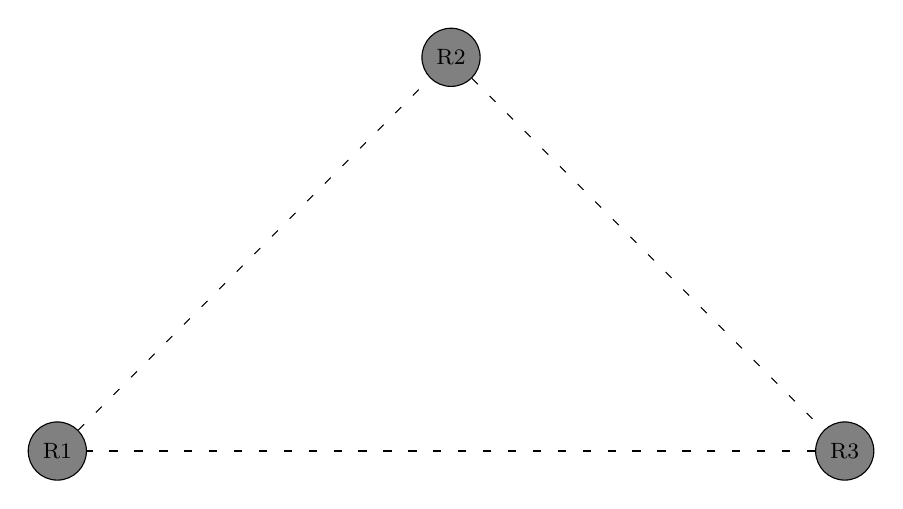
\begin{tikzpicture}[auto,node distance=3cm,on grid]
	\tikzstyle{round} = [draw,circle,minimum size=20pt,font=\footnotesize,fill=gray]
	\tikzstyle{link} = [loosely dashed]

	\node[round] at (0,0) (r1) {R1};
	\node[round] at (5,5) (r2) {R2};
	\node[round] at (10,0) (r3) {R3};

	\begin{scope}[link]
		\draw (r1) -- (r2);
		\draw (r2) -- (r3);
		\draw (r3) -- (r1);
	\end{scope}
\end{tikzpicture}



	\caption{Another figure}
	\label{figure:another}
\end{figure}

\section{Quisque arcu orci}
\label{section:lorem:quisque}

Pellentesque hendrerit aliquet placerat. Sed tincidunt lobortis eros, ut laoreet
lorem facilisis sit amet. Suspendisse ultrices, orci nec rhoncus hendrerit,
turpis augue luctus dolor, eget dignissim urna urna ac velit. Vivamus ligula
lorem, consequat vel iaculis et, lacinia in arcu. Nam imperdiet faucibus
lobortis. Ut quis libero sapien. Praesent odio est, sodales ut commodo vitae,
ultrices vel nibh. Etiam quis orci tincidunt sapien mattis aliquam. Maecenas
consequat, odio quis convallis ullamcorper, nibh justo elementum nulla, eu
molestie enim felis id neque. Sed rutrum lobortis velit, non facilisis neque
sodales et. Nunc nibh purus, gravida non ultricies in, suscipit et erat. Mauris
dui ante, fringilla vitae auctor eu, mattis a quam. Quisque at lectus
orci~\ref{table:sometable}.

\begin{table}[ht]
	\begin{center}
		\caption{Some table}
		\begin{tabular}{@{}lllr@{}}
			\toprule
			AA & BB & CC & Size (\si{\kilo\byte})  \\
			\midrule
			baz & bar & OFF & 128 \\
			aaa & dd & ON & 4 \\
			bbb & efg & OFF & 64 \\
			ccc & hij & ON & 96 \\
			\bottomrule
		\end{tabular}
		\label{table:sometable}
	\end{center}
\end{table}

Mauris risus sem, sodales quis lobortis ac, vehicula sit amet leo. Sed interdum
scelerisque tellus vitae porta. Morbi eros urna, luctus ac adipiscing ut, luctus
eleifend turpis. Sed in ligula risus, ac posuere dui. Aenean bibendum est felis.
Suspendisse a pretium quam. Sed quam lectus, semper sed pulvinar eu, condimentum
id augue.~\cite{Doe:2009}



\chapter{Summary}
\label{section:summary}

Nam dignissim facilisis velit vitae suscipit. Praesent tempor, lectus sed scelerisque consequat, nisi diam bibendum nisl, fringilla congue augue nisi et lectus. Nulla facilisi. Vestibulum elit mauris, dignissim eget tempor ac, mattis sit amet velit. Duis ultricies tincidunt mi, at ullamcorper ipsum viverra pharetra. Donec leo lectus, fringilla vel egestas vitae, hendrerit nec mauris. Pellentesque porttitor congue justo, ac viverra neque ultricies ut. Nunc sed dolor nulla, in sodales velit. Sed varius, tellus ut suscipit ultricies, risus ante tristique neque, vitae placerat mauris nibh eu metus. Maecenas metus mauris, pellentesque sed tristique ut, lacinia ac elit.

Nulla varius aliquam neque, nec porttitor diam rhoncus ut. Cum sociis natoque penatibus et magnis dis parturient montes, nascetur ridiculus mus. Duis varius tellus nec turpis ultrices in gravida dui pharetra. Nulla a felis lorem, eu facilisis quam. Proin blandit urna in nulla scelerisque sollicitudin. Aliquam feugiat, sem convallis vulputate lacinia, ligula neque sodales tellus, vel eleifend justo sapien a lectus. Aliquam nibh leo, pellentesque a posuere ac, vulputate vel mauris. Nunc dolor neque, dictum a posuere nec, scelerisque quis lectus. Ut sed tellus lectus. Nullam eu metus a leo vulputate mattis. Aliquam justo lorem, consequat ac facilisis nec, faucibus sed orci. Donec sed lacinia ligula. Fusce condimentum consectetur porta. Suspendisse et risus orci.

Cras quis nisl eu eros tristique vulputate non gravida nulla. Pellentesque metus urna, rutrum quis egestas non, iaculis sed purus. Maecenas dignissim lectus in urna tincidunt consequat. Cum sociis natoque penatibus et magnis dis parturient montes, nascetur ridiculus mus. Duis quis mauris eros, sit amet venenatis purus. Integer eleifend tempor consectetur. Aliquam sed sem justo, ut interdum sapien. Praesent pretium gravida sapien eu convallis. Sed molestie augue sed nulla tincidunt sed iaculis elit lobortis. Proin feugiat, massa eu pharetra semper, erat nulla tincidunt arcu, a posuere risus ante eu libero. Nunc scelerisque mollis sapien lobortis dignissim. In hac habitasse platea dictumst. Praesent commodo cursus arcu, eget tempor massa fringilla ut. Aenean fringilla tempus dictum.

Cras pharetra bibendum felis nec fringilla. Curabitur accumsan iaculis justo, eget imperdiet erat malesuada sed. Quisque lorem eros, feugiat sollicitudin adipiscing at, rutrum quis elit. Nulla non nisl nunc. Fusce vitae tortor non enim vestibulum suscipit in imperdiet elit. Curabitur sit amet leo purus, quis ornare dui. Suspendisse vel arcu vel diam iaculis adipiscing a sit amet mauris. Vestibulum augue magna, placerat vitae sagittis in, iaculis quis sem. Proin ut arcu pulvinar orci blandit iaculis. Etiam mauris lacus, luctus a dictum vel, rhoncus non dui. Mauris est urna, varius eget egestas a, adipiscing nec odio. Aenean iaculis nisi sed quam pretium aliquet. Quisque et mi lacus, nec porta ante. Nunc sed ante id diam hendrerit interdum in vitae eros. Ut odio ligula, commodo id volutpat non, tristique at odio.



% Fix numbering of bibliography section
\cleardoublepage
\phantomsection

\addcontentsline{toc}{chapter}{\bibname}
\printbibliography

% Appendices go here
% ------------------------------------------------------------------
% If you do not have appendices, comment out the following lines
\appendix
\chapter{Lorem ipsum}
\label{section:appendix1}

Cras pharetra bibendum felis nec fringilla. Curabitur accumsan iaculis justo, eget imperdiet erat malesuada sed. Quisque lorem eros, feugiat sollicitudin adipiscing at, rutrum quis elit. Nulla non nisl nunc. Fusce vitae tortor non enim vestibulum suscipit in imperdiet elit. Curabitur sit amet leo purus, quis ornare dui. Suspendisse vel arcu vel diam iaculis adipiscing a sit amet mauris. Vestibulum augue magna, placerat vitae sagittis in, iaculis quis sem. Proin ut arcu pulvinar orci blandit iaculis. Etiam mauris lacus, luctus a dictum vel, rhoncus non dui. Mauris est urna, varius eget egestas a, adipiscing nec odio. Aenean iaculis nisi sed quam pretium aliquet. Quisque et mi lacus, nec porta ante. Nunc sed ante id diam hendrerit interdum in vitae eros. Ut odio ligula, commodo id volutpat non, tristique at odio.



% End of document!
% ------------------------------------------------------------------
% The LastPage package automatically places a label on the last page.
% That works better than placing a label here manually, because the
% label might not go to the actual last page, if LaTeX needs to place
% floats (that is, figures, tables, and such) to the end of the
% document.
\end{document}

